\model{While Loops}

A loop is a set of instructions that are to be repeated.
All loops have three main components: \emph{initialize}, \emph{test}, and \emph{update}.
Label each of these components in the two example loops below.

\vspace{1ex}
\begin{javalst}
    // pre-test loop                         // post-test loop
    number = 1;                              number = 1;
    while (number <= 10) {                   do {
        System.out.println(number);              System.out.println(number);
        number++;                                number++;
    }                                        } while (number <= 10);
\end{javalst}

\vspace{2pt}
\hspace{3em}
\raisebox{0.5em}{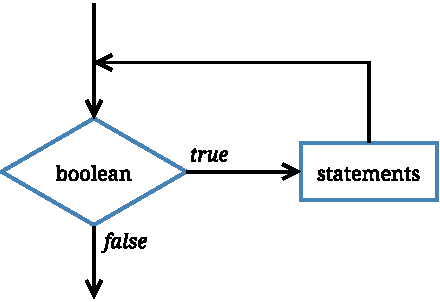
\includegraphics[height=9em]{while.pdf}}
\hspace{9em}
\raisebox{0em}{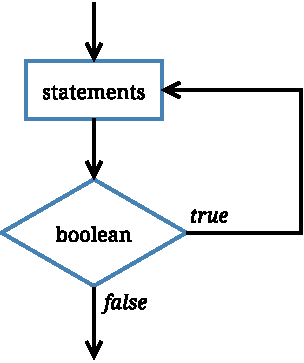
\includegraphics[height=10em]{dowhile.pdf}}


\quest{15 min}


\Q Which loop component always happens first? Why?

\begin{answer}
The initialize step; you need to tell the loop where to begin.
And variables cannot be updated until they have an initial value.
\end{answer}


\Q Explain why the \java{while} loop is called a \emph{pre-test} and the \java{do while} loop is called a \emph{post-test}.

\begin{answer}
The \texttt{while} tests its condition before the loop body, whereas the \texttt{do while} tests its condition after the loop body.
\end{answer}


\Q \label{output}
What is output (to the screen) by each loop?

\begin{answer}
They both print the numbers 1 through 10, with each number on its own line.
\end{answer}


\Q \label{value}
What is the final value of \java{number} at the end of each loop?

\begin{answer}
At the end of each loop, the value of \java{number} is 11.
\end{answer}


\Q What is output if you swap the \java{println} and \java{number++} statements?

\begin{answer}
Both loops print the values 2 through 11 instead.
\end{answer}


\Q What is the output if you remove the \java{number++} statement?

\begin{answer}
Both loops will print the value 1 forever, since \java{number} never reaches the stopping condition.
\end{answer}


\Q \label{do99}
What is output by the loop below?

\begin{minipage}{0.49\textwidth}
\begin{javalst}
    number = 99;
    do {
        System.out.println(number);
        number++;
    } while (number <= 10);
    System.out.println(number);
\end{javalst}
\end{minipage}
\hfill
\begin{minipage}{0.49\textwidth}
\begin{answer}[5em]
It will print the numbers 99 and 100; the \texttt{do while} loop does not repeat since 99 is greather than 10.
\end{answer}
\end{minipage}
\vspace{1ex}


\Q What is the output of the following loop? (And what mistake was made?)

\begin{minipage}{0.49\textwidth}
\begin{javalst}
    i = 0;
    while (i < 3) 
        System.out.println("i = " + i);
        i = i + 1;
\end{javalst}
\end{minipage}
\hfill
\begin{minipage}{0.49\textwidth}
\begin{answer}
It will print \texttt{"i = 0"} forever. Without braces, the loop only executes the first statement, and ~\java{i = i + 1;} is never reached.
\end{answer}
\end{minipage}
\vspace{1ex}


\Q What is the difference between a \java{while} statement and an \java{if} statement?

\begin{answer}
They identical syntax and a similar meaning; the only difference is a \texttt{while} statement repeats the code between its braces as long as the condition is \texttt{true}.
\end{answer}
